\section{Das Semesterticket -- die neue Freiheit}

\begin{center}
	\includegraphics[width=\textwidth, height=0.22\textheight]{res/bus_und_bahn.pdf}
\end{center}
\begin{multicols*}{2}
\begin{figure*}[t]
	\subsection{Geltungsbereich des NRW-Tickets}
	% XXX Jedes Jahr Regionalverkehrsplan aktualisieren
	% Quelle Regionalverkehrsplan:
	% https://www.vrr.de/de/fahrten/busundbahn/verkehrsplaene/index.html
	% http://busse-und-bahnen.nrw.de/service-organisation/service/nrw-regionalverkehrsplan/
	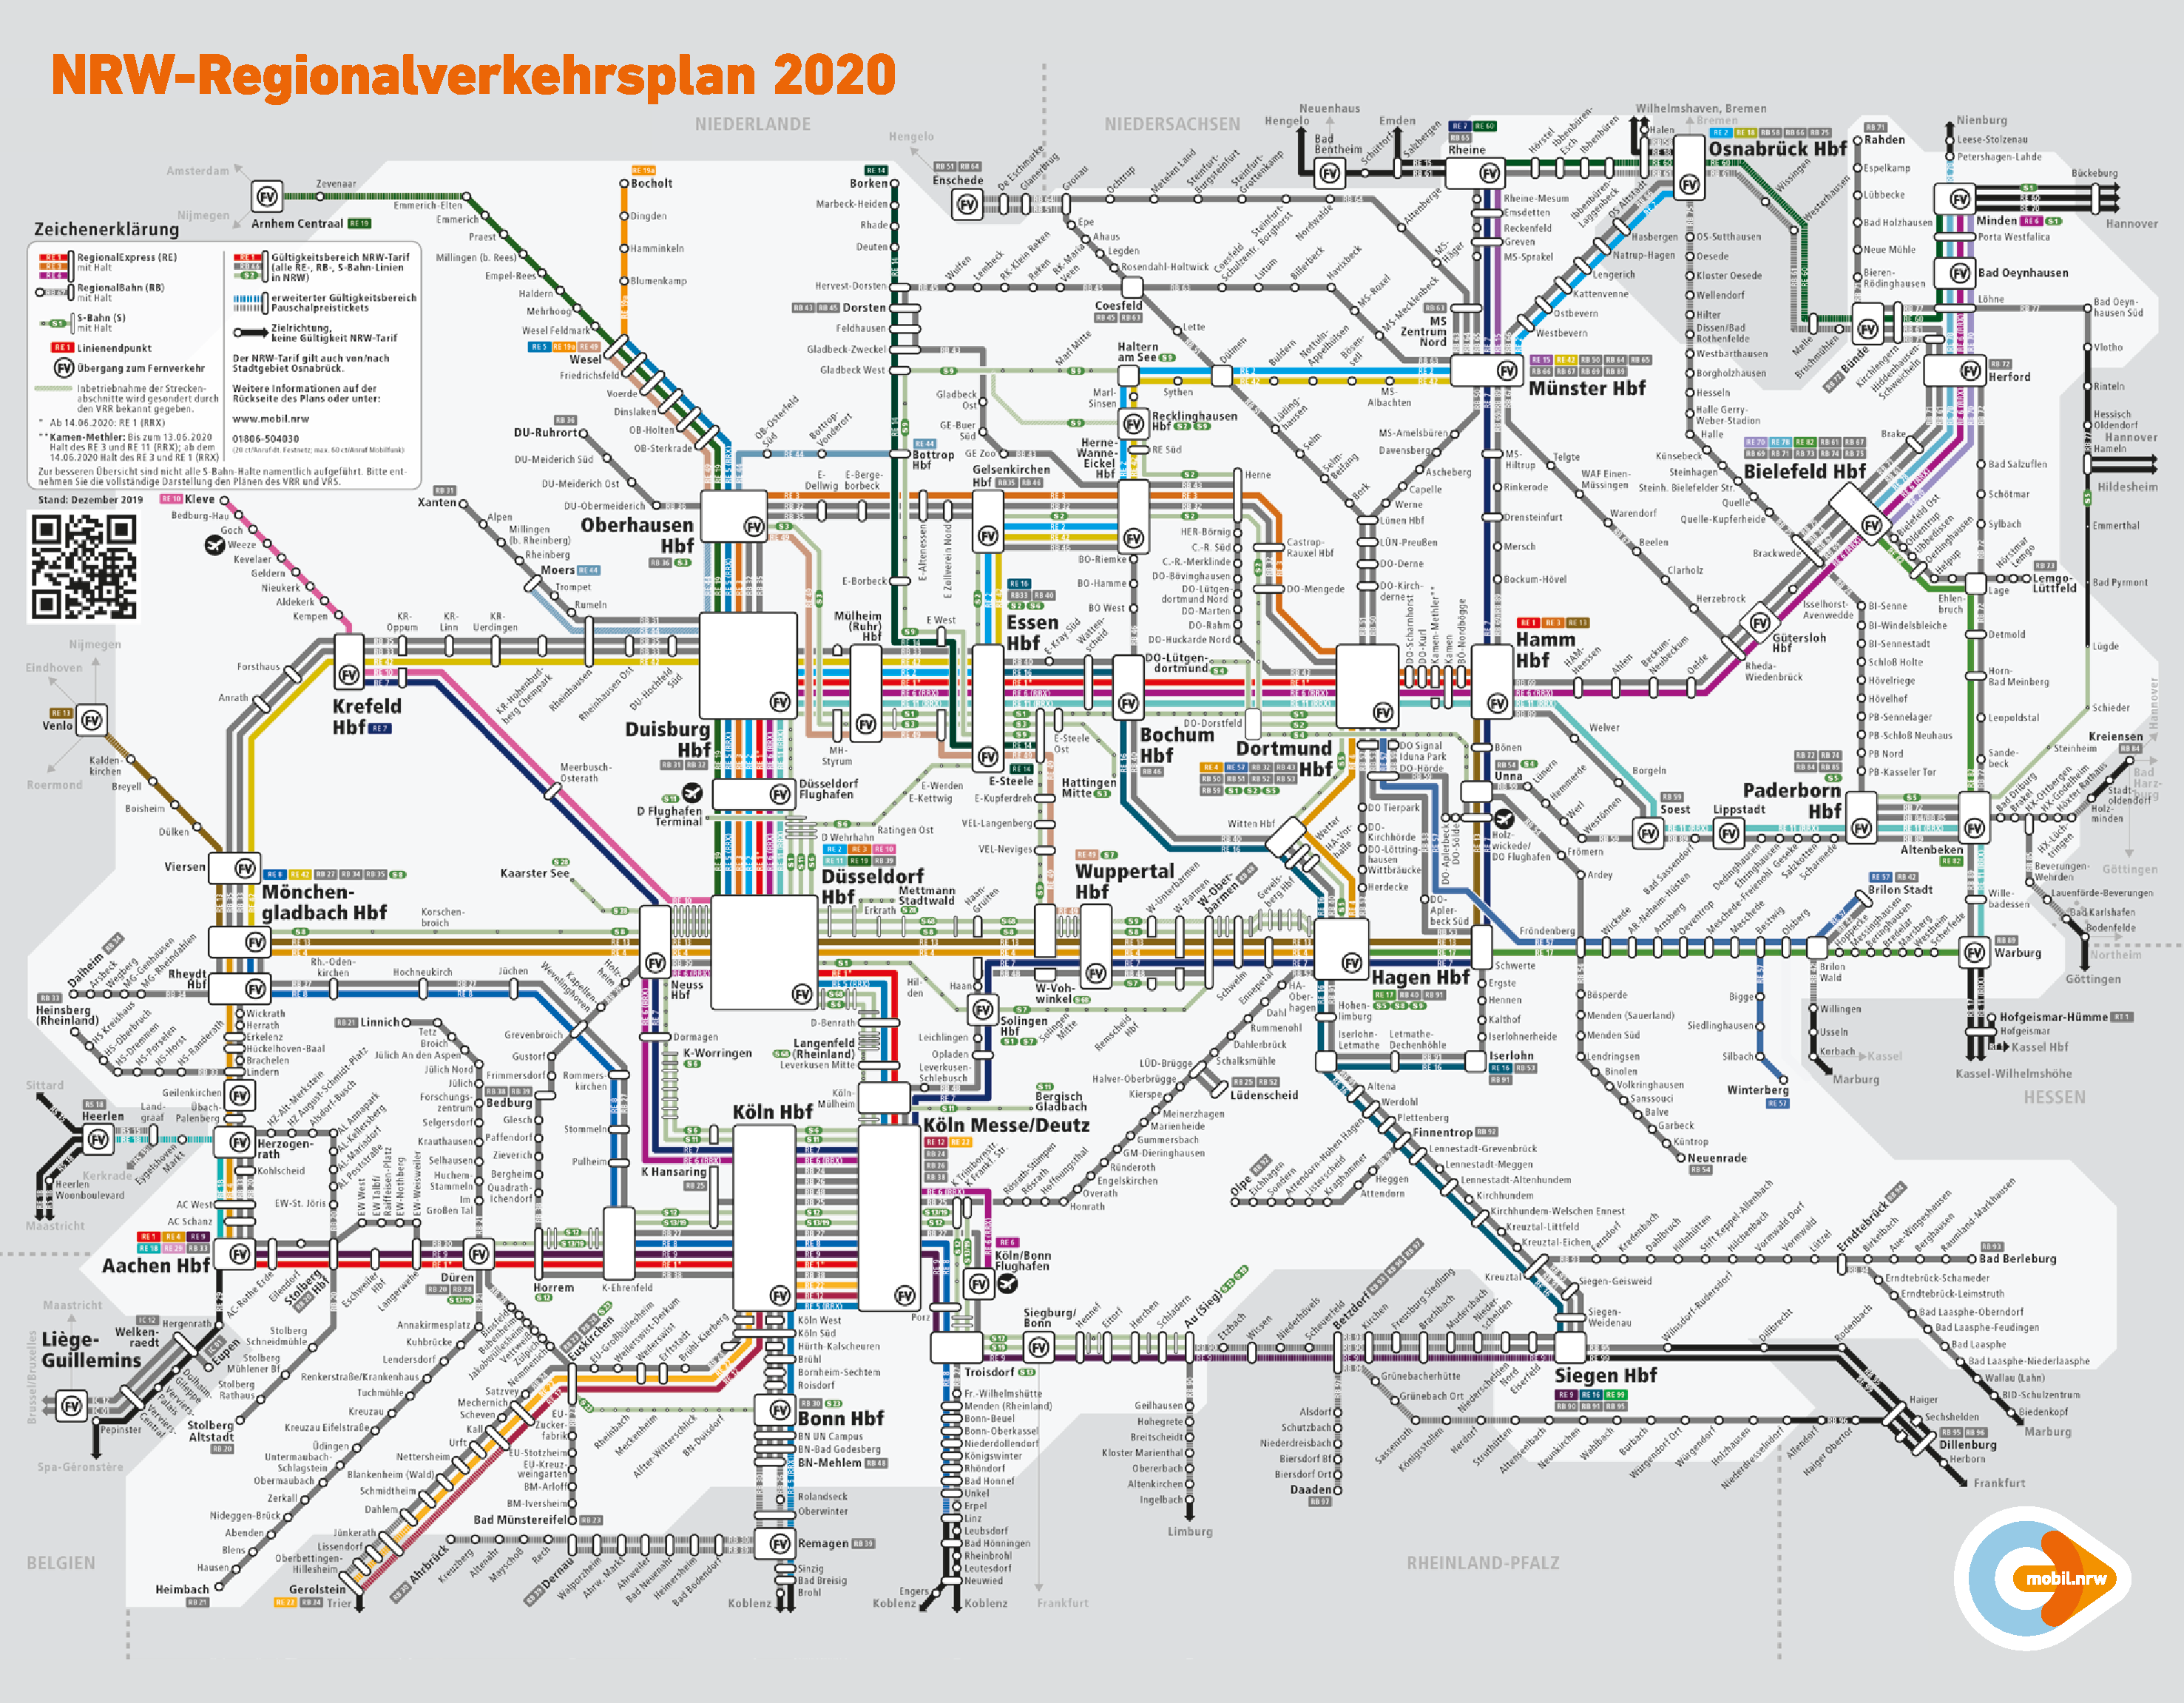
\includegraphics[width=\textwidth]{res/regionalverkehrsplan_nrw.pdf}
\end{figure*}
\textbf{Früher hab' ich mal geglaubt, das Semesterticket sei nur für den Weg nach Hause bestimmt, aber da lag ich nicht ganz richtig: Das Semesterticket~(SeTi) kann noch viel mehr.}

\includegraphics[width=\columnwidth]{res/semesterticket.pdf}

Vor Beginn jedes neuen Semesters bekommst du eine freundliche E-Mail, in der du dazu aufgefordert wirst, dich für das kommende Semester zurückzumelden. In dieser Mail ist auch ein Link enthalten, in dem du auswählen musst, ob du dein Semesterticket in Papierform zugeschickt bekommen oder es digital herunterladen möchtest. Beides ist leider nicht möglich.
Ohne einen gültigen Lichtbildausweis ist das Semesterticket nicht gültig.
Die meisten Busfahrer sehen es nicht als Verstoß an, wenn man mal keinen Lichtbildausweis bei sich trägt, doch spätestens, wenn du das Semesterticket für Fahrten mit der Bahn verwendest, musst du einen gültigen Ausweis bei dir tragen.

Der Universität Münster (bzw.\ dem AStA) ist es vor einigen Jahren nach langen Diskussionen und einer Urabstimmung gelungen, mit der Deutschen Bahn einen Vertrag über ein NRW-Ticket abzuschließen.
Daher darfst du dich im kompletten Nahverkehr in NRW bewegen.
Zusätzlich gilt das Ticket auch für ausgewählte Bahn-Strecken außerhalb von NRW, z.\,B.\ von Münster nach Osnabrück, Enschede (Niederlande) und Lingen oder auch von Lengerich (Westfahlen) nach Osnabrück (Details siehe Webseite im "Ersti-Überlebenszettel" bzw.\ am Artikelende).

Nahverkehr bedeutet, dass du alle Busse, Straßenbahnen, U-Bahnen, S-Bahnen sowie alle Regionalbahnen -- RegionalExpress~(RE), RegionalBahn~(RB), und alle privaten Bahnen -- im Raum Nordrhein-Westfalen benutzen darfst.
Natürlich zählt der Fernverkehr -- InterCity~(IC) und InterCityExpress~(ICE) -- nicht zum Nahverkehr.

Solltest du mal mit der Bahn unterwegs sein und dein Semesterticket liegt zu Hause, ist das zwar ärgerlich, aber kein Beinbruch.
Zunächst wirst du vom Schaffner als "Schwarzfahrer" aufgeschrieben, mit dem Vorbehalt einer \SI{60}{\euro}-Strafe.
Dieses Schreiben musst du dann zusammen mit deinem Semesterticket am Schalter in Münster vorzeigen und musst nur eine Bearbeitungsgebühr in Höhe von ungefähr \SI{10}{\euro} bezahlen.
Ärgerlich, aber besser, als die ganzen \SI{60}{\euro} zu zahlen.

Solltest du mal per Anschlusszug über die Grenzen des NRW-/Semestertickets hinaus fahren wollen, denk daran, das nötige Ticket rechtzeitig (am besten gleich als "Viererticket") zu lösen, denn Nachlösen im Zug ist mittlerweile nicht mehr möglich.

Es ist von Zeit zu Zeit ganz ratsam, sich über die Optionen deines Semestertickets neu zu informieren.
So wurde zum Beispiel vor einiger Zeit geändert, dass du in Bussen \emph{im Stadtgebiet Münster sowie in Hamm, Rheine und Bocholt} ab 19~Uhr sowie an Wochenenden und Feiertagen ganztägig eine weitere Person oder ein Fahrrad mitnehmen darfst (gilt nicht für Bahnverbindungen).
Aufgrund des begrenzten Platzangebots entscheidet der Busfahrer, ob ein Fahrrad mitgenommen werden darf oder nicht.
Auch neu ist, dass das Semesterticket für Erstsemester bereits einen Monat vor Semesterbeginn gilt.

\subsection{Das Kultursemesterticket}
Seit es 2015 durch eine Urabstimmung in der Studierendenschaft eingeführt wurde, gibt es neben dem Semesterticket das sogenannte Kultursemesterticket. Dieses wird ähnlich wie das Semesterticket aus den Semesterbeiträgen finanziert und erlaubt Studierenden, viele kulturelle Einrichtungen in Münster vergünstigt oder sogar kostenlos zu besuchen. Dies handelt der AStA jeweils direkt mit der ensprechenden Einrichtung aus – der Grad der Vergünstigung kann daher stark variieren. So bieten z.\,B. das Museum für Lackkunst und der Literaturverein freien Eintritt, während das Theater Münster ein festes Kontingent an Freikarten und kostenlose Restplätze anbietet und das GOP Variet\'e für einige Veranstaltungstermine jede Woche Sonderpreise für Studierende hat. Fußballfans dürfte interessieren, das der AStA für jedes Heimspiel des SC Preußen Münster 50 Freikarten bekommt, die man sich beim AStA sichern kann.
Die vollständige Übersicht gibt es unter
\vspace{-1ex}
\begin{center}
	\url{https://www.asta.ms/kultursemesterticket}
\end{center}

\smallskip

\begin{center}
	\includegraphics[width=\columnwidth, height=0.12\textheight]{res/bushaltestelle.pdf}

	{\bfseries
	Aktualisierte Infos zum SeTi gibt es unter\\
	\url{https://www.stadtwerke-muenster.de/privatkunden/busverkehr/tickets/semesterticket/}}
	
	(weitere Links findet ihr im "Ersti-Überlebenszettel" auf Seite~\pageref{dpü} dieser Ersti-$\Phi$bel)
\end{center}

\fibelsig{Andreas G., Simon}
\end{multicols*}
